% §5 Experimental Results
% Status: Revised 2026-03-25 — full results from E1–E7 on RTX 5060 + MI300X.

\section{Experimental Results}
\label{sec:results}

This section presents results from all seven experiments in order of increasing
workload irregularity. Each subsection identifies the dominant abstraction
failure or success patterns observed and connects them to the empirical taxonomy
developed in Section~\ref{sec:taxonomy}. Section~\ref{subsec:crosscutting}
synthesises cross-cutting findings into the portability matrix that underpins
the decision framework (Section~\ref{sec:framework}).

% ===================================================================
\subsection{E1: STREAM Triad --- Memory-Bound Baseline}
\label{subsec:e1}
% ===================================================================

STREAM Triad ($A[i] = B[i] + s \cdot C[i]$) is the best-case scenario for any
portability framework: perfectly regular, embarrassingly parallel, and
bandwidth-bound. Figure~\ref{fig:e1-crossplatform} shows cross-platform PPC
at the large problem size ($N = 2^{28}$).

\begin{figure}[t]
\centering
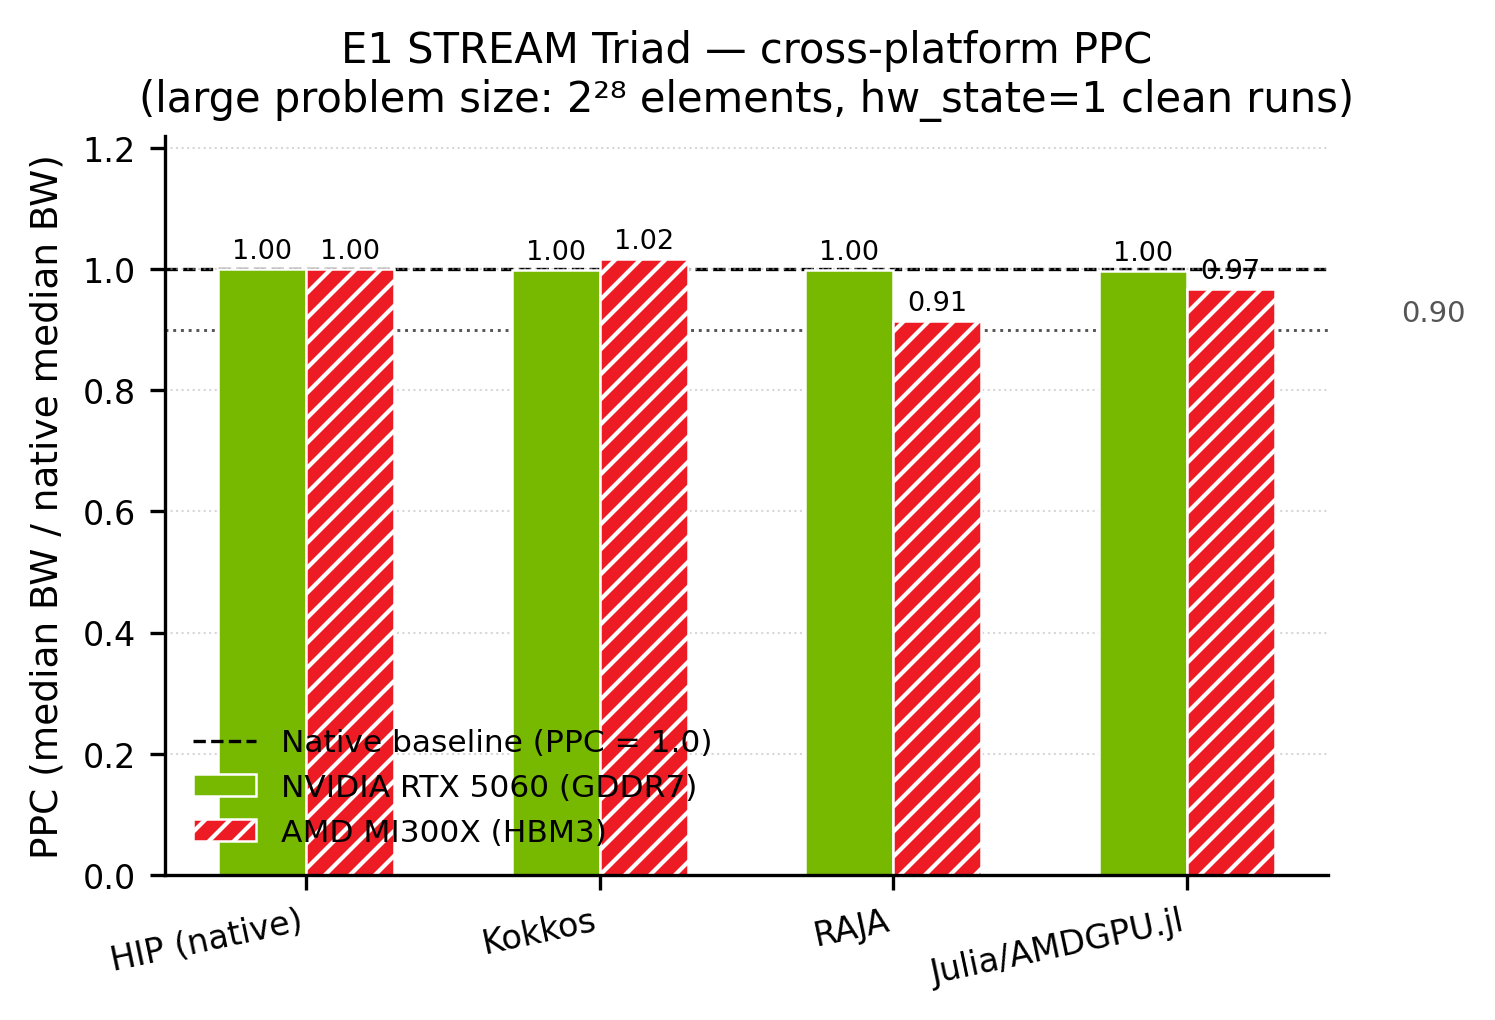
\includegraphics[width=\columnwidth]{figures/e1/fig8_e1_crossplatform_ppc.png}
\caption{E1 STREAM Triad: cross-platform PPC at $N = 2^{28}$.
All abstractions achieve PPC $\geq 0.91$ on both platforms.}
\label{fig:e1-crossplatform}
\end{figure}

All four abstractions deliver near-native bandwidth at large $N$: Kokkos
(1.00/1.02), RAJA (1.00/0.91), and Julia (1.00/0.97) on NVIDIA/AMD
respectively. Cross-platform $\varphi \geq 0.95$ for all abstractions,
confirming that \emph{memory-bound portability at large problem sizes is a
solved problem}.

However, the picture changes at small $N$. Figure~\ref{fig:e1-amd-size} shows
AMD MI300X bandwidth as a function of problem size.

\begin{figure}[t]
\centering
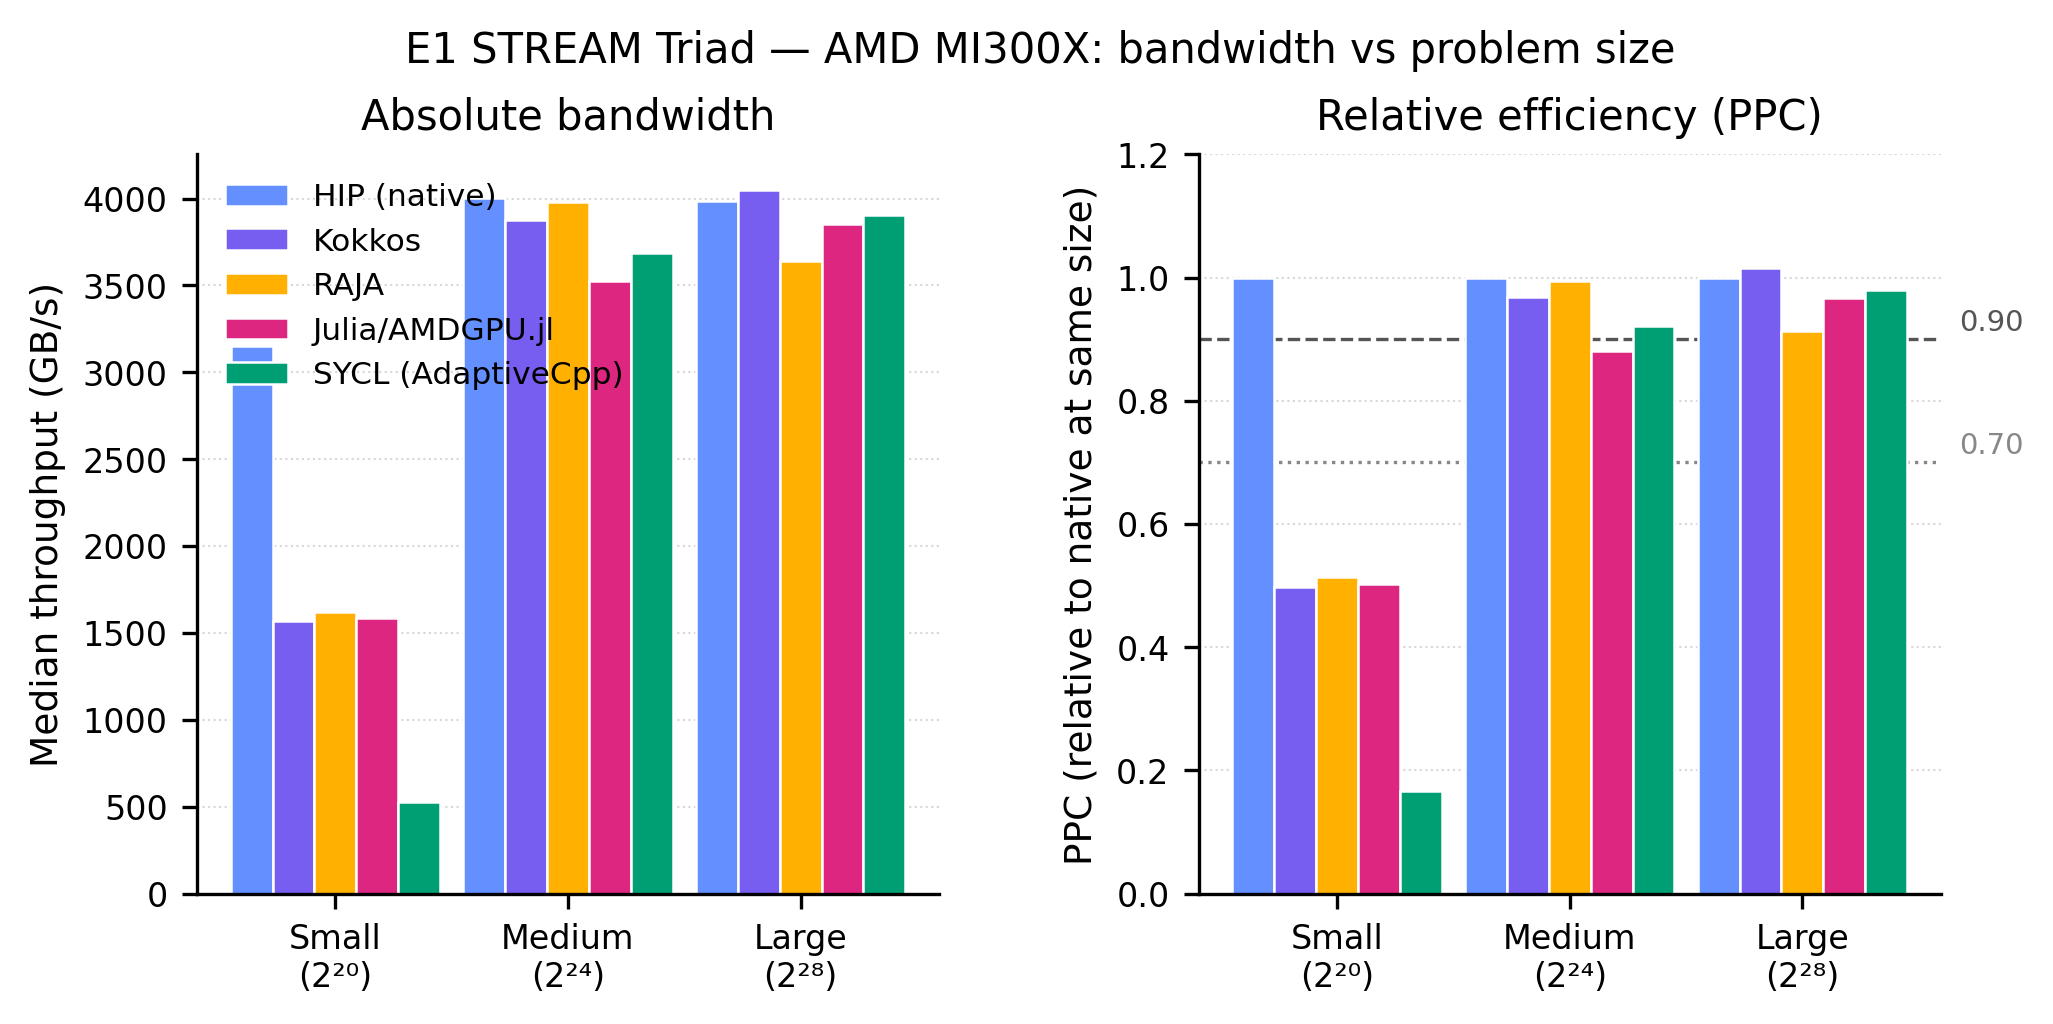
\includegraphics[width=\columnwidth]{figures/e1/fig7_e1_amd_size_sensitivity.png}
\caption{E1 STREAM Triad on AMD MI300X: bandwidth and efficiency vs.\
problem size. SYCL collapses to 0.167 efficiency at small $N$ (P001).}
\label{fig:e1-amd-size}
\end{figure}

SYCL drops to $\eta = 0.167$ at $N = 2^{20}$ on AMD (527 vs.\ 3154\,GB/s
native)---the canonical example of pattern P001 (Launch Overhead Dominance).
The HSA dispatch overhead ($\approx$19\,\textmu{}s) exceeds the kernel
execution time at this problem size. Julia similarly drops to $\eta = 0.55$
at small $N$ on AMD ($\approx$4\,\textmu{}s dispatch overhead). At large $N$,
both recover to $> 0.96$, confirming that the penalty is purely
overhead-driven and amortises with problem size.

% ===================================================================
\subsection{E2: Dense Matrix Multiplication --- API Expressivity Gap}
\label{subsec:e2}
% ===================================================================

DGEMM is compute-bound ($\sim$16--64\,FLOP/byte) and requires shared-memory
tiling for optimal performance. This experiment exposes the most consequential
failure mode in our dataset: pattern P004 (API Expressivity Gap).

\begin{figure*}[t]
\centering
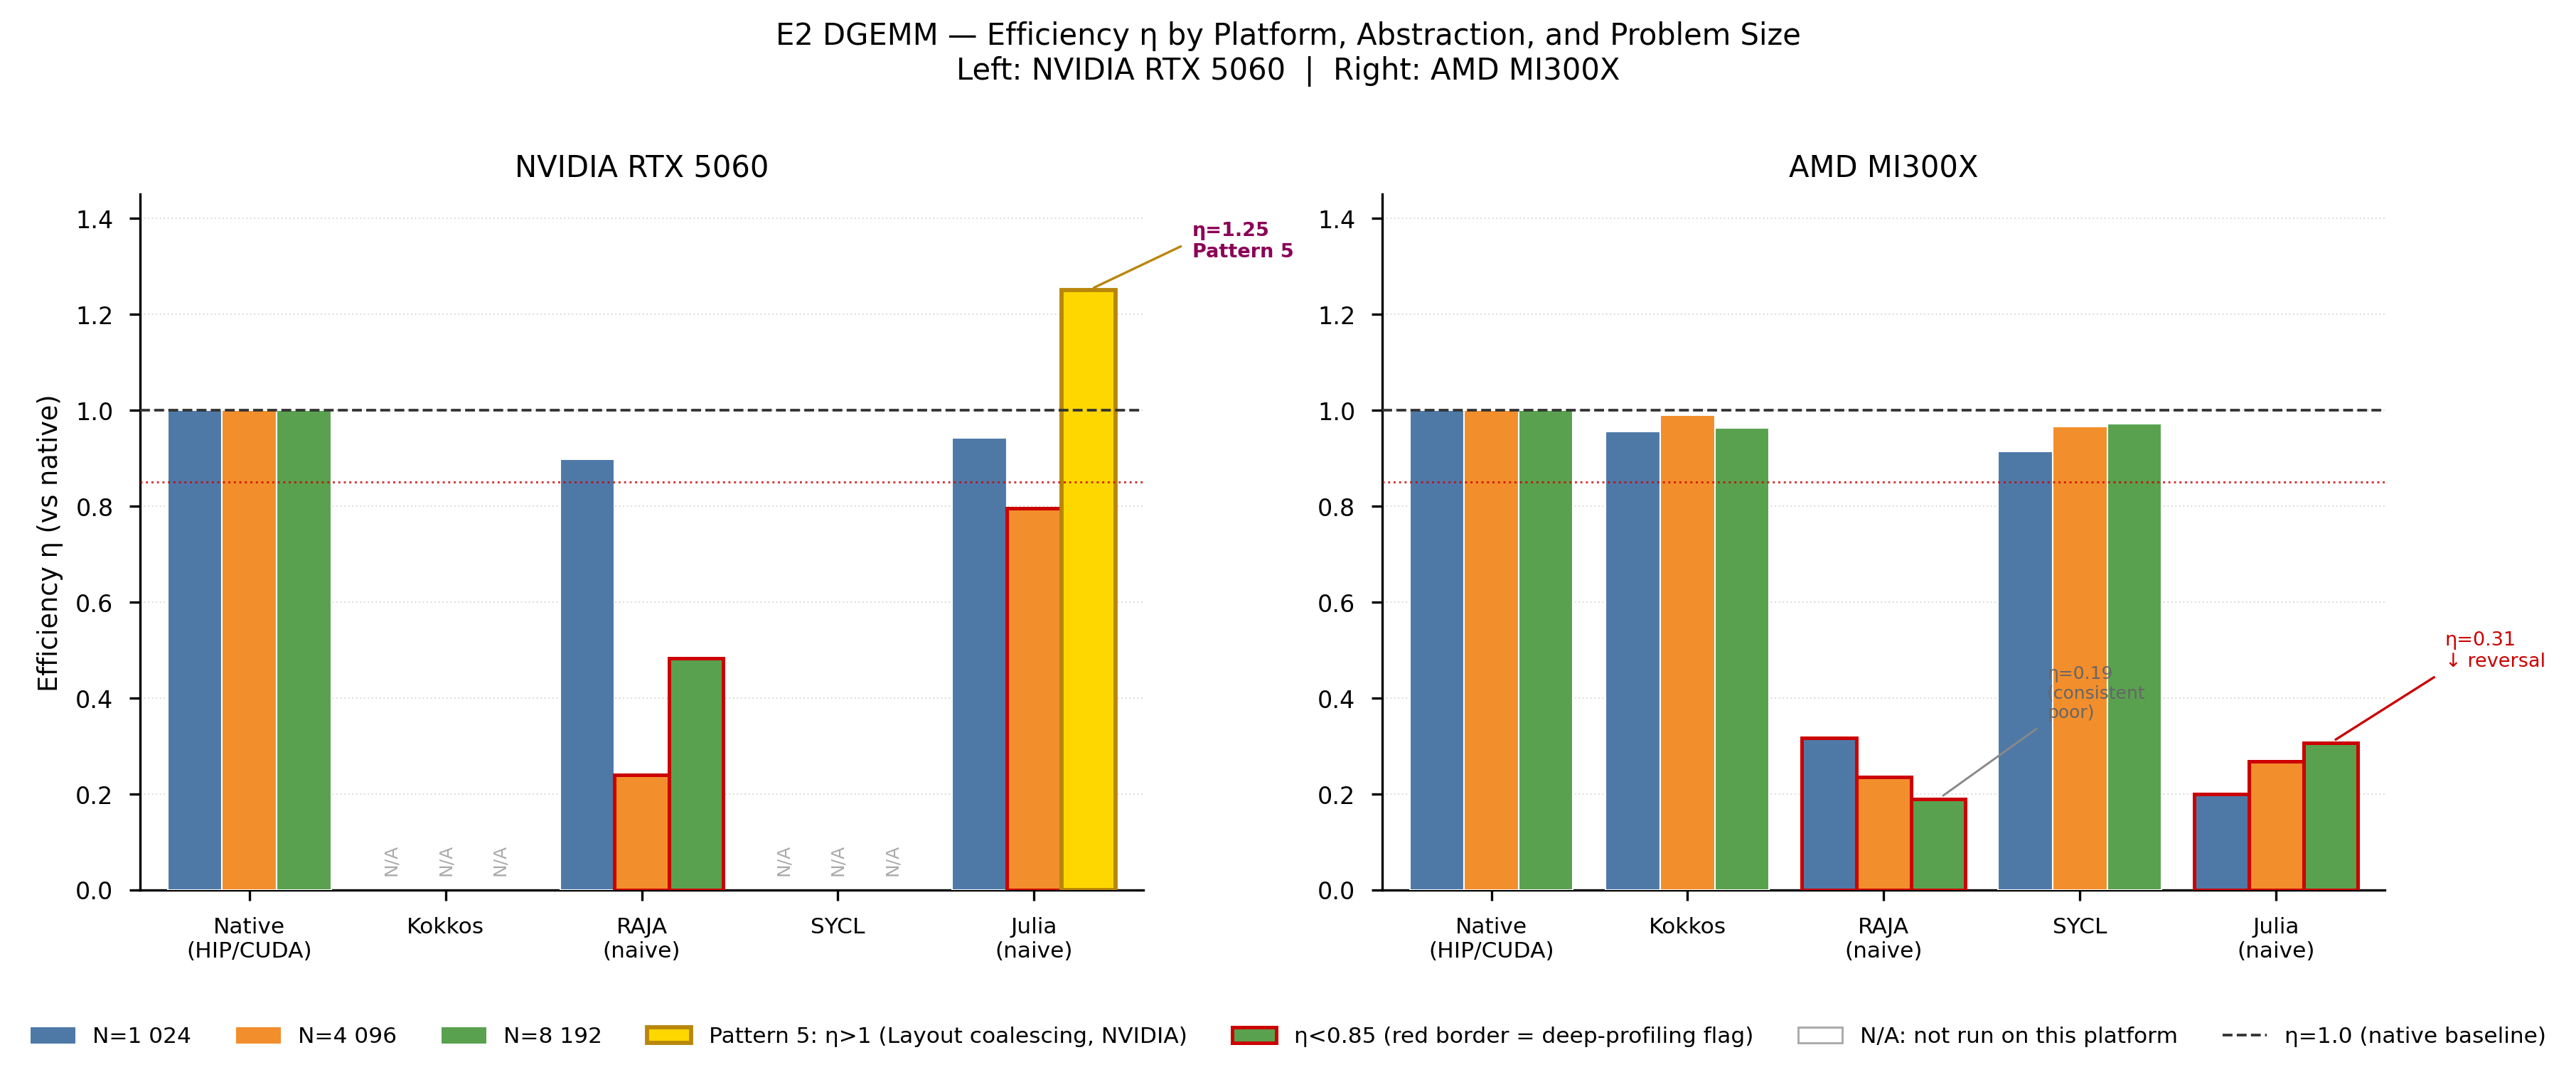
\includegraphics[width=\textwidth]{figures/e2/fig_e2_efficiency_multiplatform.png}
\caption{E2 DGEMM: efficiency by abstraction, platform, and problem size.
Left: NVIDIA RTX~5060. Right: AMD MI300X. Red borders indicate configurations
flagged for deep profiling ($\eta < 0.85$). Julia exceeds native on NVIDIA
(P005) but collapses on AMD. RAJA and Julia lack shared-memory tiling on both
platforms (P004).}
\label{fig:e2-multiplatform}
\end{figure*}

Figure~\ref{fig:e2-multiplatform} reveals a sharp divide. Abstractions with
shared-memory access---Kokkos (\texttt{TeamPolicy}: $\eta = 0.963$ on AMD)
and SYCL (\texttt{local\_accessor}: $\eta = 0.972$)---achieve near-native
performance. Abstractions without it---RAJA (\texttt{forall}: $\eta = 0.189$
at large $N$ on AMD) and Julia (\texttt{@cuda}: $\eta = 0.306$)---are
catastrophically poor.

RAJA's degradation is size-\emph{independent}: $\eta$ drops from 0.316
(small) to 0.236 (medium) to 0.189 (large) on AMD, confirming that the root
cause is algorithmic ($O(N^3)$ global-memory traffic vs.\ $O(N^2)$ with
tiling), not launch overhead. This is pattern P004: the API cannot express
the optimal algorithm.

Julia on NVIDIA tells a different story. At large $N$, Julia achieves
$\eta = 1.25$---exceeding native CUDA. This is pattern P005 (Layout-Induced
Coalescing Advantage): Julia's column-major \texttt{CuArray} storage produces
superior warp-level memory access patterns for this kernel. However, this
advantage is \emph{architecture-specific}: on AMD MI300X, the same Julia
kernel delivers only $\eta = 0.31$, a platform-generation reversal relative
to Godoy et al.'s finding of $\eta > 0.90$ on CDNA2
(MI250X)~\cite{Godoy2023}.

\begin{figure}[t]
\centering
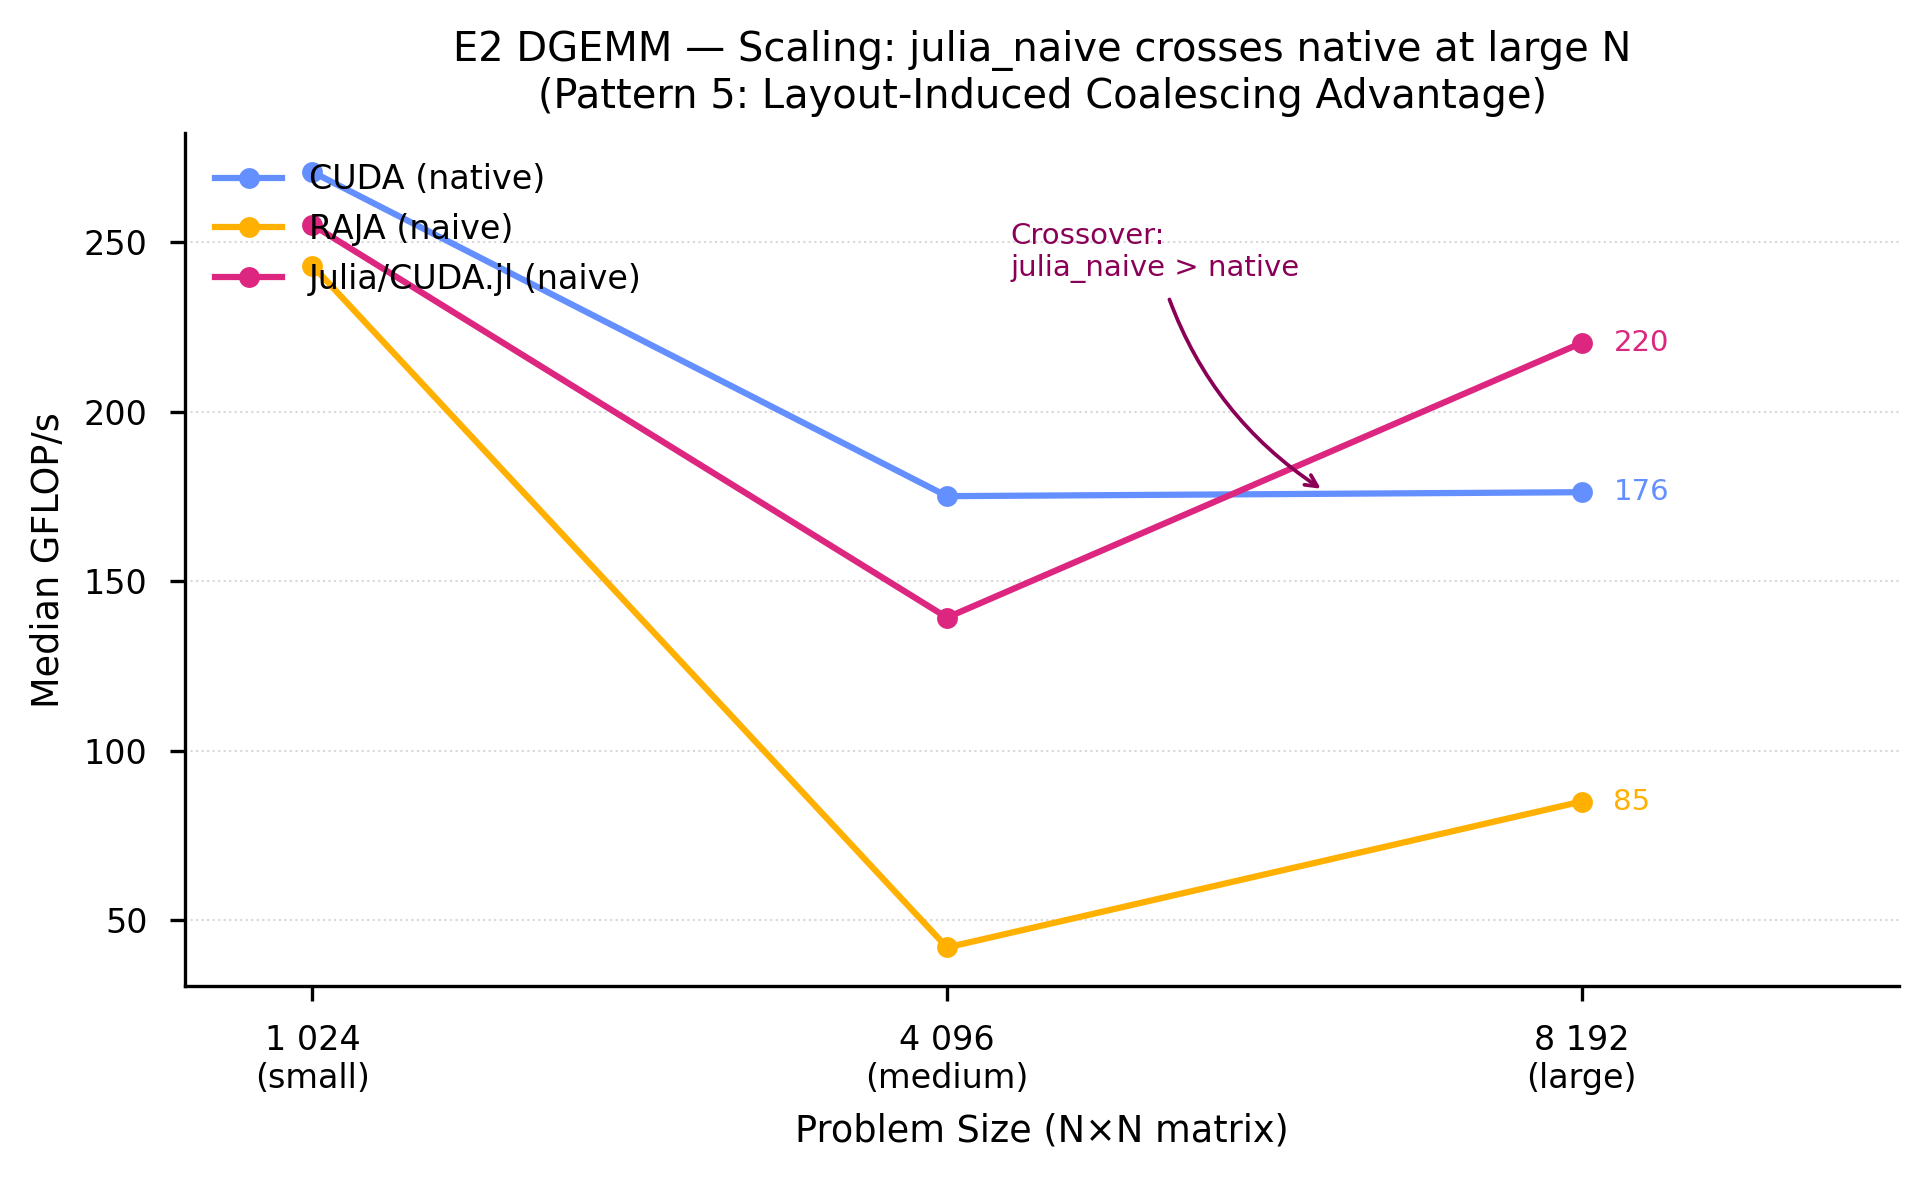
\includegraphics[width=\columnwidth]{figures/e2/fig3_e2_scaling_crossover.png}
\caption{E2 DGEMM: scaling behaviour across problem sizes. Julia's P005
layout advantage scales with $N$ on NVIDIA but is absent on AMD.}
\label{fig:e2-scaling}
\end{figure}

Cross-platform portability scores confirm the severity: $\varphi_\text{raja\_naive} = 0.272$ (worst in the dataset) and
$\varphi_\text{julia\_naive} = 0.492$. The thermal contamination protocol
(Section~\ref{subsec:thermal}) was essential here: the raw
\texttt{raja\_naive}/medium efficiency of $\eta = 0.24$ on RTX~5060 was
corrected to $\eta = 0.66$ after fresh-state profiling revealed a
$2.76\times$ thermal ratio---the residual gap is genuine P004 overhead, not
measurement artefact.

% ===================================================================
\subsection{E3: 3D Stencil --- Tiling Policy Overhead}
\label{subsec:e3}
% ===================================================================

The 7-point Jacobi stencil is memory-bound (AI $\approx 0.203$\,FLOP/byte)
and tests multi-dimensional indexing abstractions.
Figure~\ref{fig:e3-multiplatform} shows efficiency on both platforms across
four problem sizes, with the $N = 512^3$ results authoritative (exceeds
MI300X L2 cache, forcing the DRAM-bound regime).

\begin{figure*}[t]
\centering
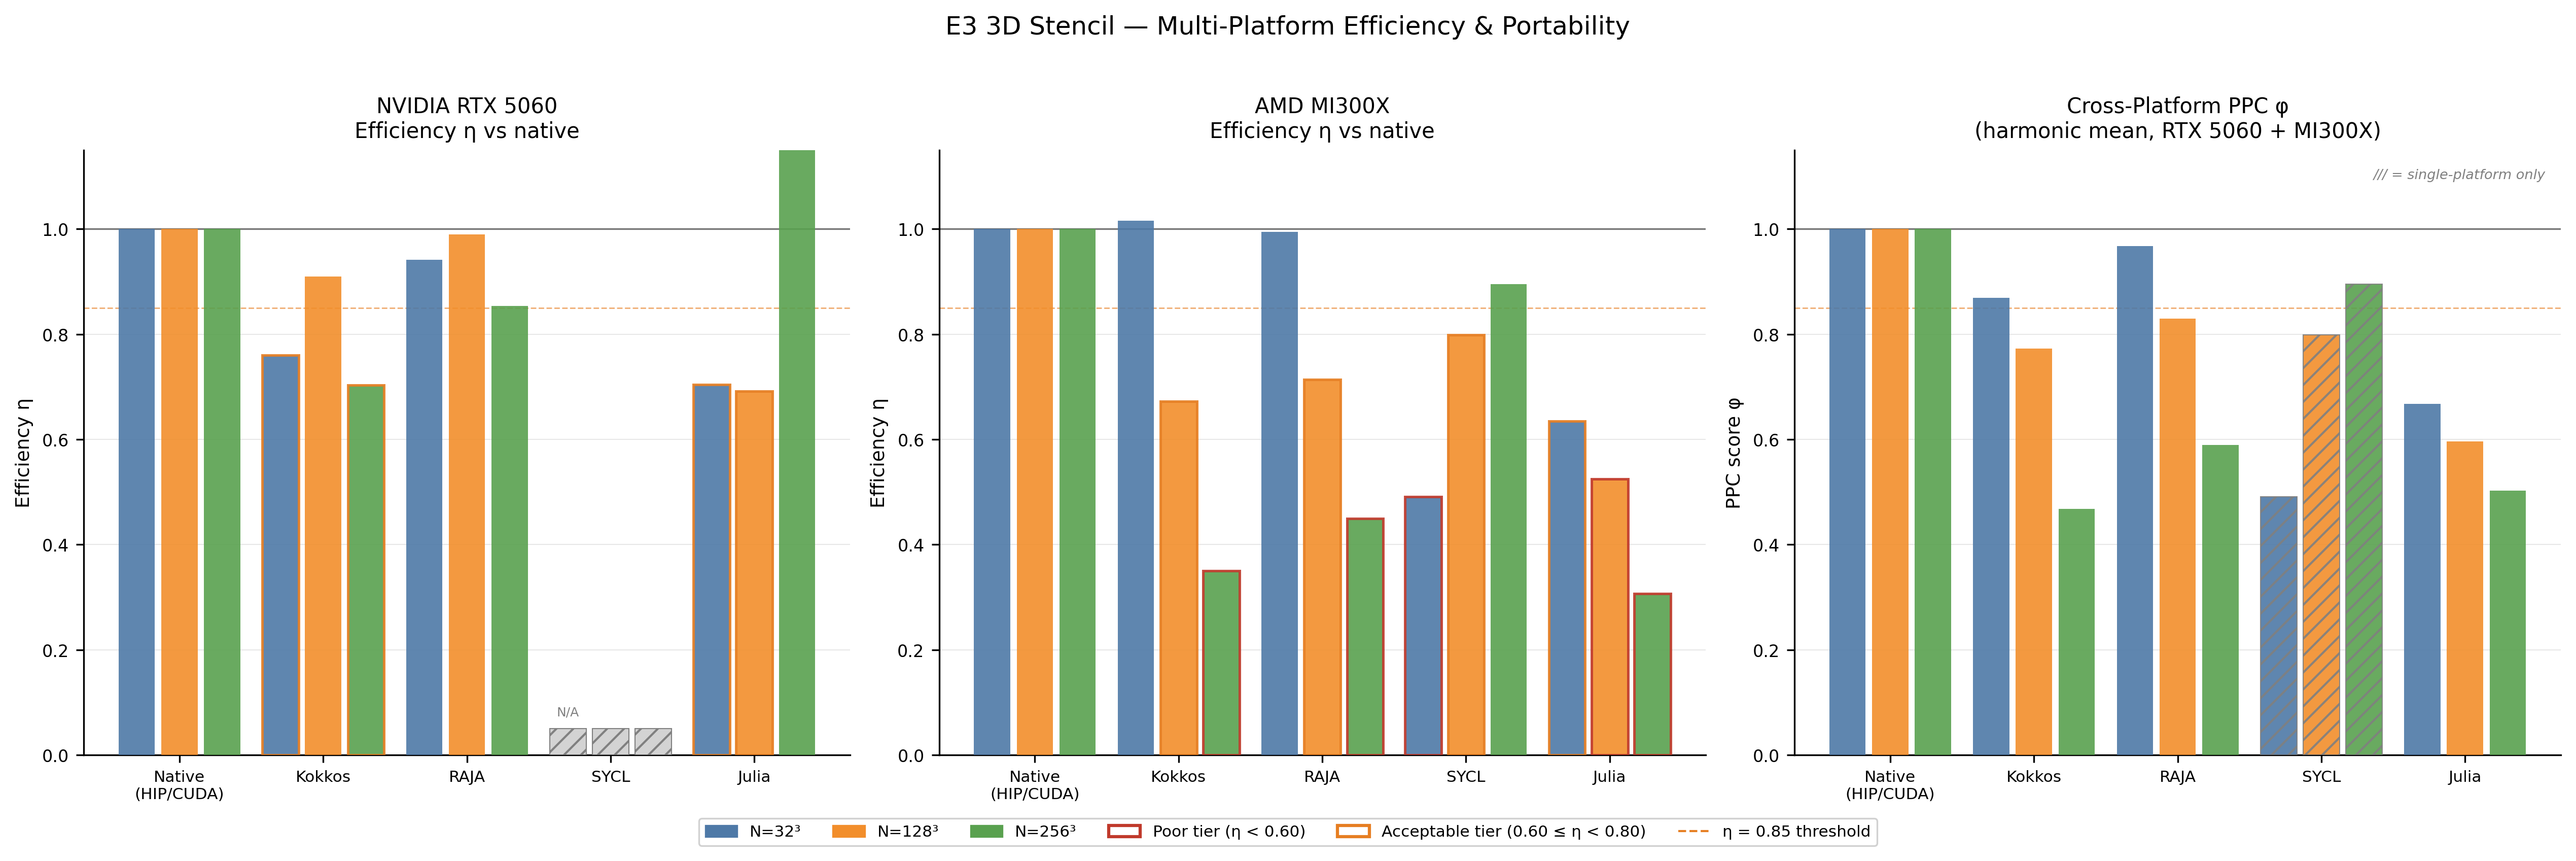
\includegraphics[width=\textwidth]{figures/e3/fig13_e3_efficiency_multiplatform.png}
\caption{E3 3D Stencil: efficiency on NVIDIA (left), AMD (centre), and
cross-platform $\varphi$ (right). SYCL achieves 98.7\% native on AMD MI300X
at $N = 512^3$---the best portability result in the dataset. Kokkos collapses
to 42\% due to \texttt{MDRangePolicy} code generation overhead (P006).}
\label{fig:e3-multiplatform}
\end{figure*}

SYCL achieves $\eta = 0.987$ on AMD at $N = 512^3$ (9{,}340\,GB/s vs.\
9{,}462\,GB/s native)---the single best portability layer result in the
entire dataset. The SYCL kernel uses a single \texttt{nd\_range} dispatch
with no \texttt{MDRangePolicy}-style boundary masking, generating clean
vectorised code.

Kokkos, by contrast, achieves only $\eta = 0.423$ on the same platform and
problem size. Investigation revealed that this is pattern P006 (Tiling Policy
Overhead): Kokkos' \texttt{MDRangePolicy} generates boundary-checking
conditionals at tile edges that dominate execution time for the 7-point
stencil's low arithmetic intensity. Enabling the wave64 execution path
recovered only 3\% of the gap, confirming that the bottleneck is code
generation quality, not warp-width mismatch.

RAJA ($\eta = 0.711$) outperforms Kokkos on this kernel because its simpler
loop-level abstraction avoids \texttt{MDRangePolicy}. Julia ($\eta = 0.466$)
exhibits unstable, bimodal timing distributions on AMD, suggesting JIT
recompilation events during timed runs.

% ===================================================================
\subsection{E4: SpMV --- Load Imbalance Amplification}
\label{subsec:e4}
% ===================================================================

Sparse matrix-vector multiplication in CSR format tests how abstractions handle
irregular memory access. We evaluate three matrix classes: structured (Laplacian),
power-law (Pareto $\gamma = 2.5$), and random (Erd\H{o}s--R\'enyi).
Figure~\ref{fig:e4-heatmap} shows the efficiency heatmap at large $N$.

\begin{figure}[t]
\centering
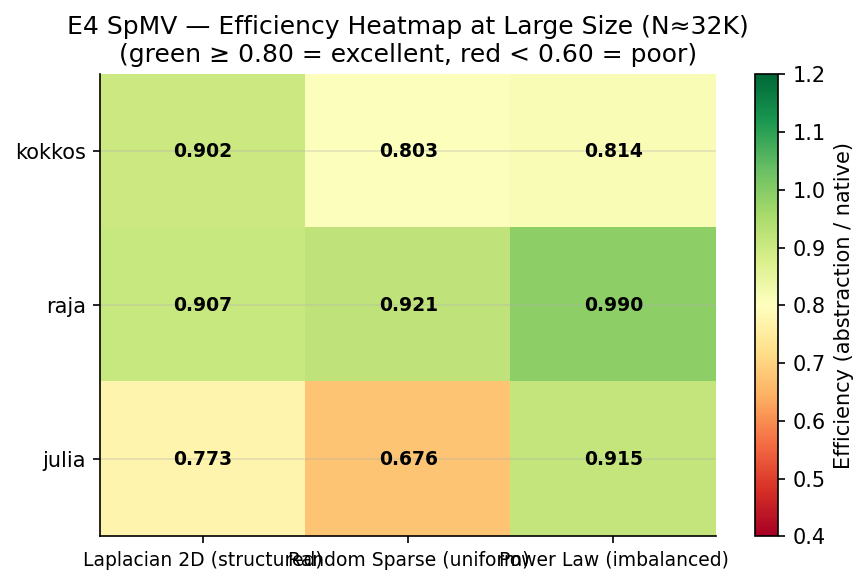
\includegraphics[width=\columnwidth]{figures/e4/fig14_e4_efficiency_heatmap.png}
\caption{E4 SpMV: efficiency heatmap at large $N$ ($N = 32$K). Green
cells ($\geq 0.80$) indicate excellent portability; red cells ($< 0.60$)
indicate poor. The power-law column is systematically redder than the
structured column, confirming P007.}
\label{fig:e4-heatmap}
\end{figure}

Pattern P007 (Load Imbalance Amplification) is validated by comparing Julia on
structured vs.\ power-law matrices at small $N$: $\eta = 0.561$ (Laplacian)
vs.\ $\eta = 0.449$ (power-law). The same kernel, same $N$, but the
power-law degree distribution ($\sigma = 2.5$) creates a 20\% compound
penalty by amplifying the per-launch overhead through load-imbalanced
wavefronts. At large $N$, all abstractions recover to $\geq 0.80$ as
overhead amortises, though the load-imbalance effect persists: Kokkos drops
from 0.902 (Laplacian) to 0.803 (power-law) even at large $N$. RAJA is less
affected (0.907 $\to$ 0.921), suggesting that its simpler dispatch path is
more tolerant of irregular workloads.

% ===================================================================
\subsection{E5: SpTRSV --- Level-Set Dispatch Amplification}
\label{subsec:e5}
% ===================================================================

Sparse triangular solve requires level-set scheduling: the matrix is
decomposed into levels of independent rows, with one kernel launch per level.
This produces $O(n_\text{levels})$ launches per solve, making per-launch
overhead the dominant performance factor. Figure~\ref{fig:e5-efficiency}
shows efficiency across both platforms.

\begin{figure*}[t]
\centering
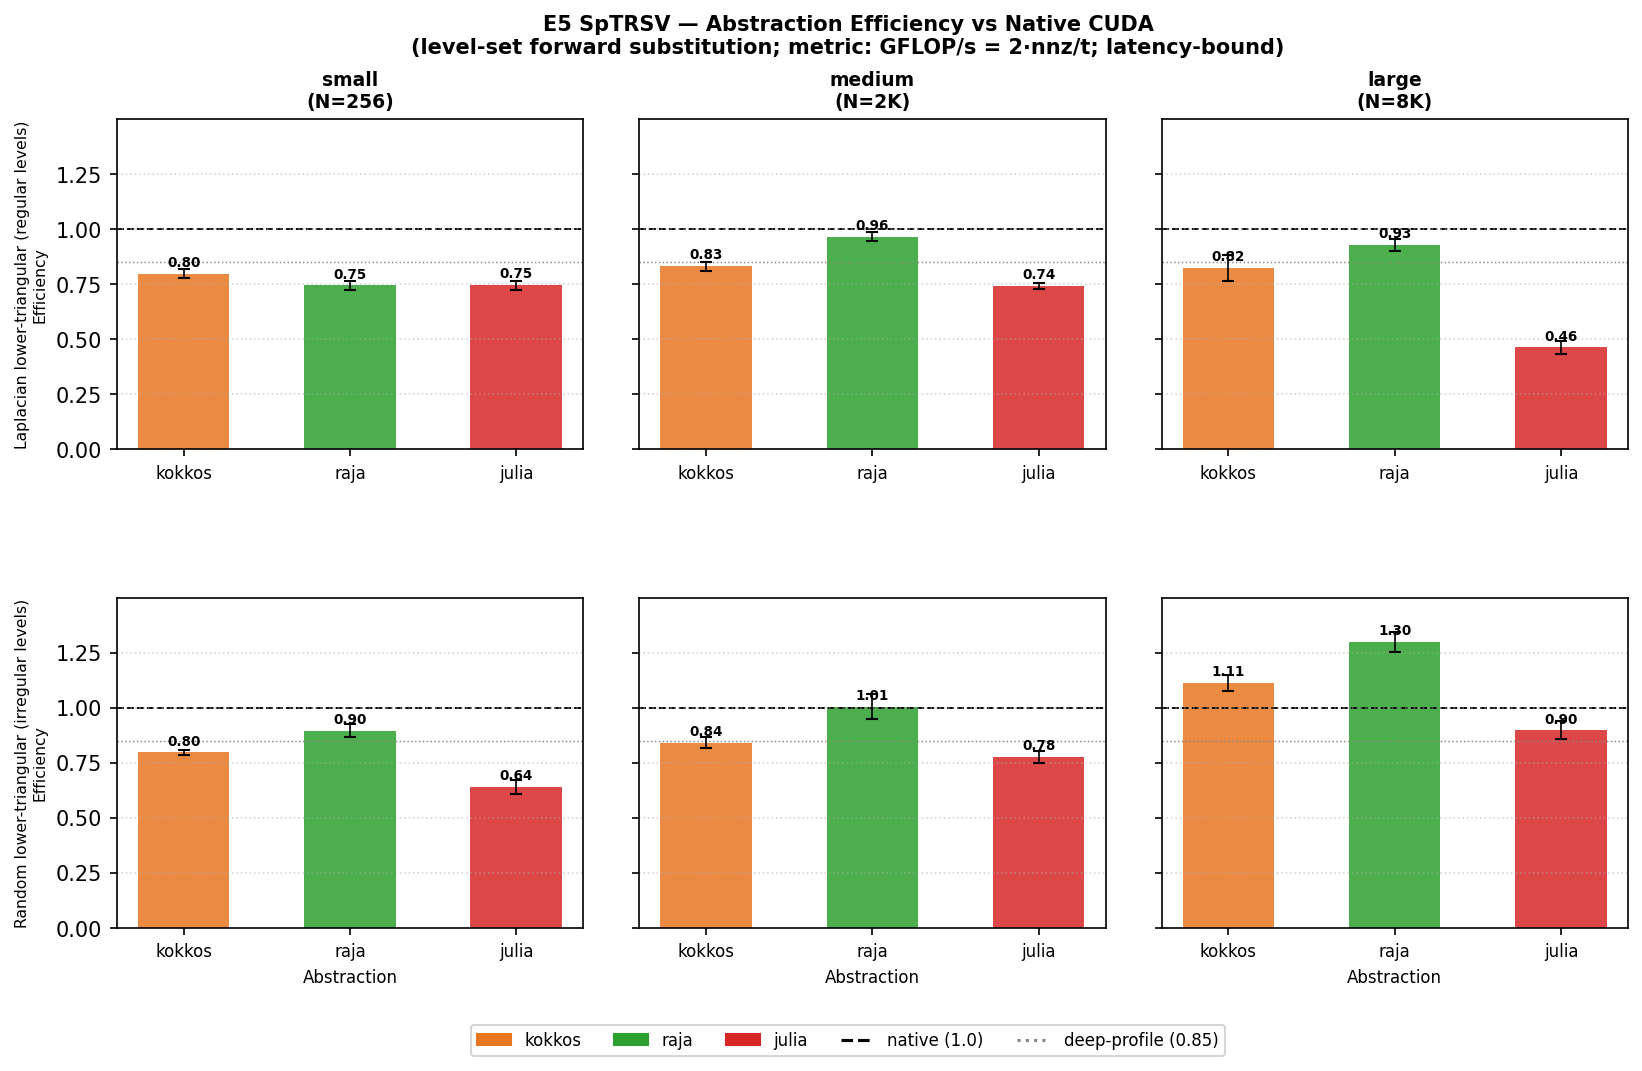
\includegraphics[width=\textwidth]{figures/e5/fig19_e5_efficiency_by_matrix.png}
\caption{E5 SpTRSV: efficiency by matrix type and size. Top row: NVIDIA
RTX~5060. Bottom row: AMD MI300X. RAJA and Kokkos exceed native at large $N$
on random matrices (inverse P008). Julia and SYCL are poor on narrow-level
Laplacian matrices (P008).}
\label{fig:e5-efficiency}
\end{figure*}

This experiment provides the strongest quantitative validation of pattern P008
(Level-Set Dispatch Amplification). The Laplacian matrix at large $N$ has
$n_\text{levels} = 181$ with minimum level width of 1 row
(Figure~\ref{fig:e5-levels}), creating a near-sequential execution pattern
regardless of abstraction.

\begin{figure}[t]
\centering
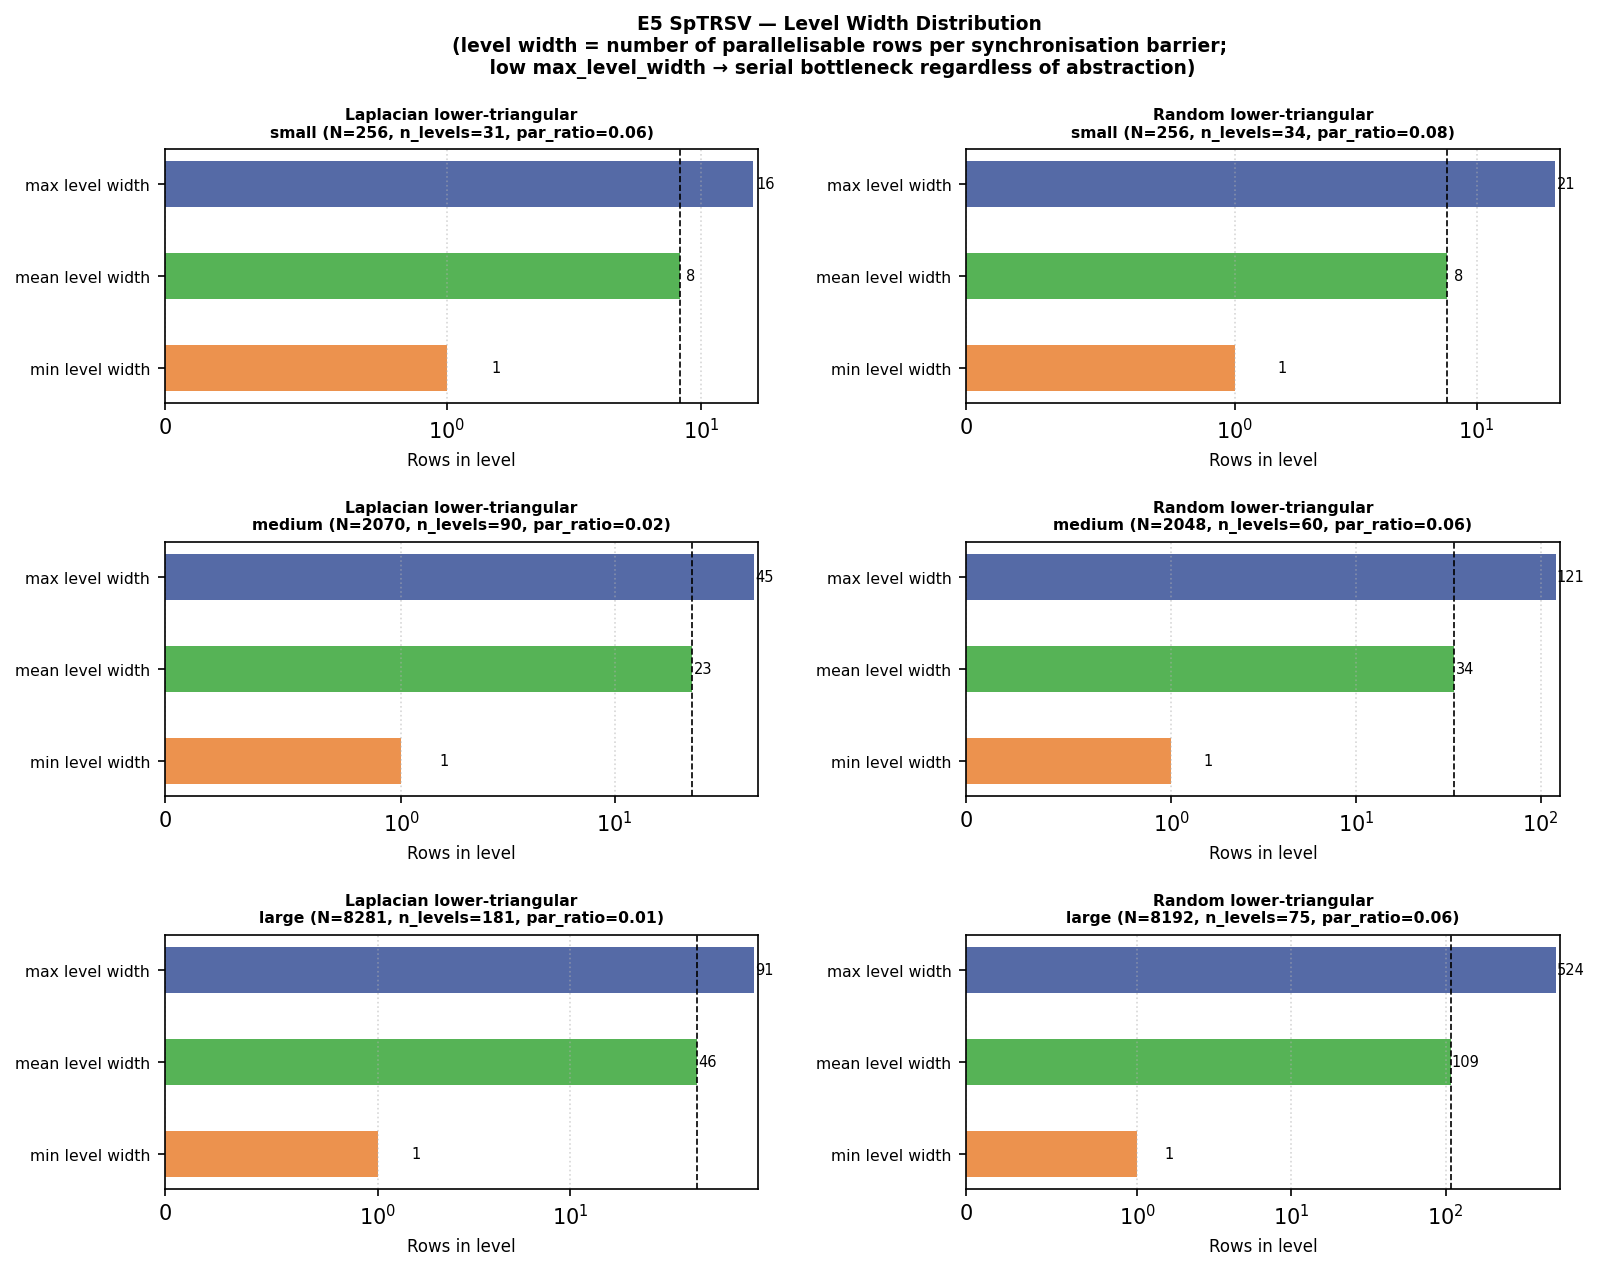
\includegraphics[width=\columnwidth]{figures/e5/fig20_e5_level_structure.png}
\caption{E5 SpTRSV: level width distributions. Laplacian matrices (left)
have narrow levels ($\min = 1$ row) requiring 181 launches at large $N$.
Random matrices (right) have wider levels ($\text{mean} = 109$ rows) with
only 75 launches.}
\label{fig:e5-levels}
\end{figure}

SYCL on AMD Laplacian/large achieves $\eta = 0.490$---exactly matching the
decision framework prediction of $\text{PPC} = 0.490$ from rule R2
(Section~\ref{sec:framework}), computed as $n_\text{levels} \times
\text{overhead}_\text{SYCL/HSA} / T_\text{compute}$. Julia on NVIDIA
Laplacian/large achieves $\eta = 0.464$, consistent with
$181 \times 25\,\text{\textmu{}s} = 4.5\,\text{ms}$ accumulated dispatch
overhead against $\sim$22.6\,\textmu{}s compute per level.

An inverse pattern emerges on random matrices with wide levels: RAJA achieves
$\eta = 1.299$ on RTX~5060 random/large, and Kokkos achieves $\eta = 1.113$.
Here, the abstraction's parallel reduction primitive outperforms the native
serial accumulation within each level---a genuine abstraction
\emph{advantage}, not merely overhead amortisation.

A cross-platform reversal is also observed: Julia on AMD ($\eta = 0.897$ for
random/large) outperforms Julia on NVIDIA ($\eta = 0.464$ for
Laplacian/large), because AMDGPU.jl's per-launch overhead ($\sim$4\,\textmu{}s)
is lower than CUDA.jl's ($\sim$7\,\textmu{}s).

% ===================================================================
\subsection{E6: Breadth-First Search --- Extreme Irregularity}
\label{subsec:e6}
% ===================================================================

Level-synchronous BFS represents the stress test for portability frameworks:
extreme load imbalance, control-flow divergence, and atomic operations.
Figure~\ref{fig:e6-efficiency} shows efficiency across graph types.

\begin{figure*}[t]
\centering
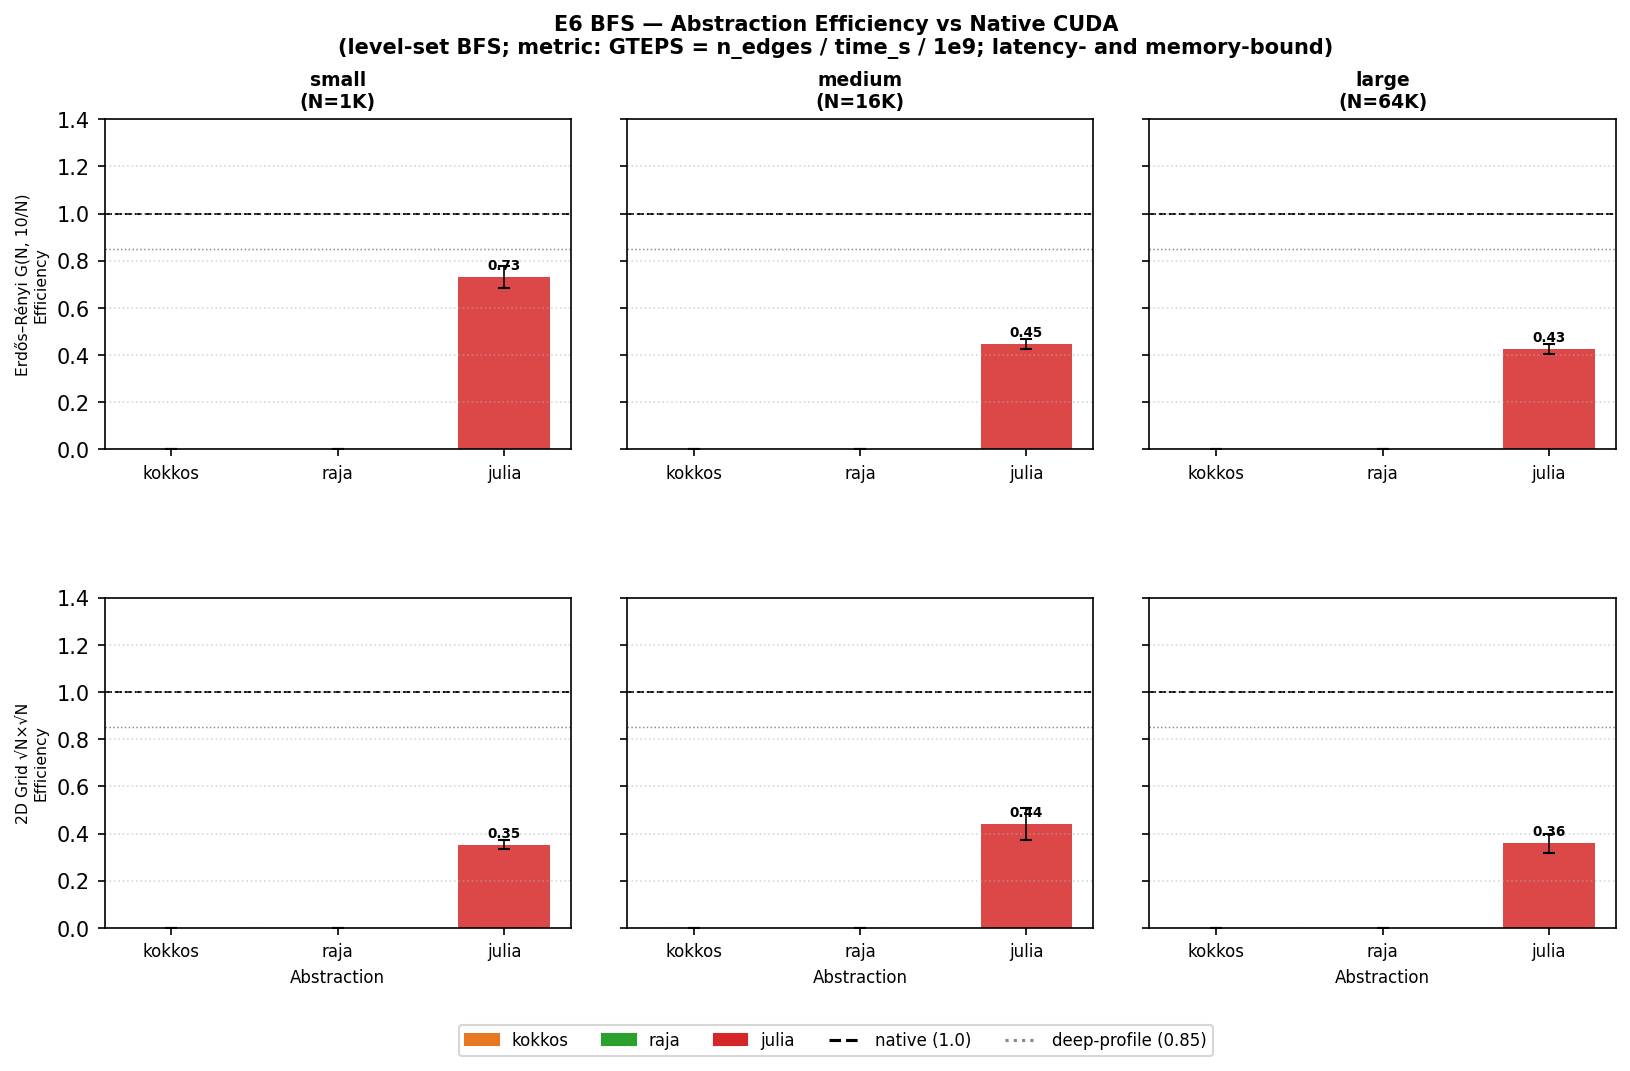
\includegraphics[width=\textwidth]{figures/e6/fig23_e6_efficiency_by_graph.png}
\caption{E6 BFS: efficiency by graph type and size. Top: NVIDIA RTX~5060.
Bottom: AMD MI300X. Kokkos exceeds native by $332\times$ on 2D grid (AMD,
large)---an algorithmic difference, not an abstraction efficiency gain.
Julia achieves only 5--6\% of native.}
\label{fig:e6-efficiency}
\end{figure*}

The most striking result is Kokkos on the AMD 2D grid at large $N$:
1.43\,GTEPS vs.\ native's 0.0043\,GTEPS---a $332\times$ speedup. However,
this is \textbf{not} an abstraction success story. The native HIP baseline
uses \texttt{thrust::copy\_if} to scan all $N = 65{,}536$ vertices per level,
while Kokkos implements a worklist that scans only the frontier. The two
implementations use fundamentally different algorithms; the comparison measures
algorithmic quality, not abstraction overhead. A fair comparison would require
the native baseline to use the same worklist strategy.

Julia achieves only 5--6\% of native performance. BFS requires multiple
sub-kernels per level (scatter, prefix sum, gather), each incurring Julia's
dispatch overhead. With $\sim$267\,\textmu{}s per level (vs.\ $\sim$25\,\textmu{}s
for SpTRSV's single kernel per level), this is an extreme instance of P008
compounded by multi-kernel dispatch.

SYCL achieves $\sim$30\% on AMD---better than Julia due to fewer sub-kernels
per level, but still dominated by HSA dispatch amplification. RAJA achieves
60--86\%, benefiting partially from its reduction primitives.

% ===================================================================
\subsection{E7: N-Body Force Calculation --- Dispatch Amortisation}
\label{subsec:e7}
% ===================================================================

The Lennard-Jones N-body force calculation uses CSR neighbour lists with a
cutoff radius. Unlike E5 and E6, this is a \emph{single-kernel} workload:
one force-computation kernel per timestep, with 100 timesteps per
measurement. Figure~\ref{fig:e7-efficiency} shows the dispatch amortisation
curve.

\begin{figure}[t]
\centering
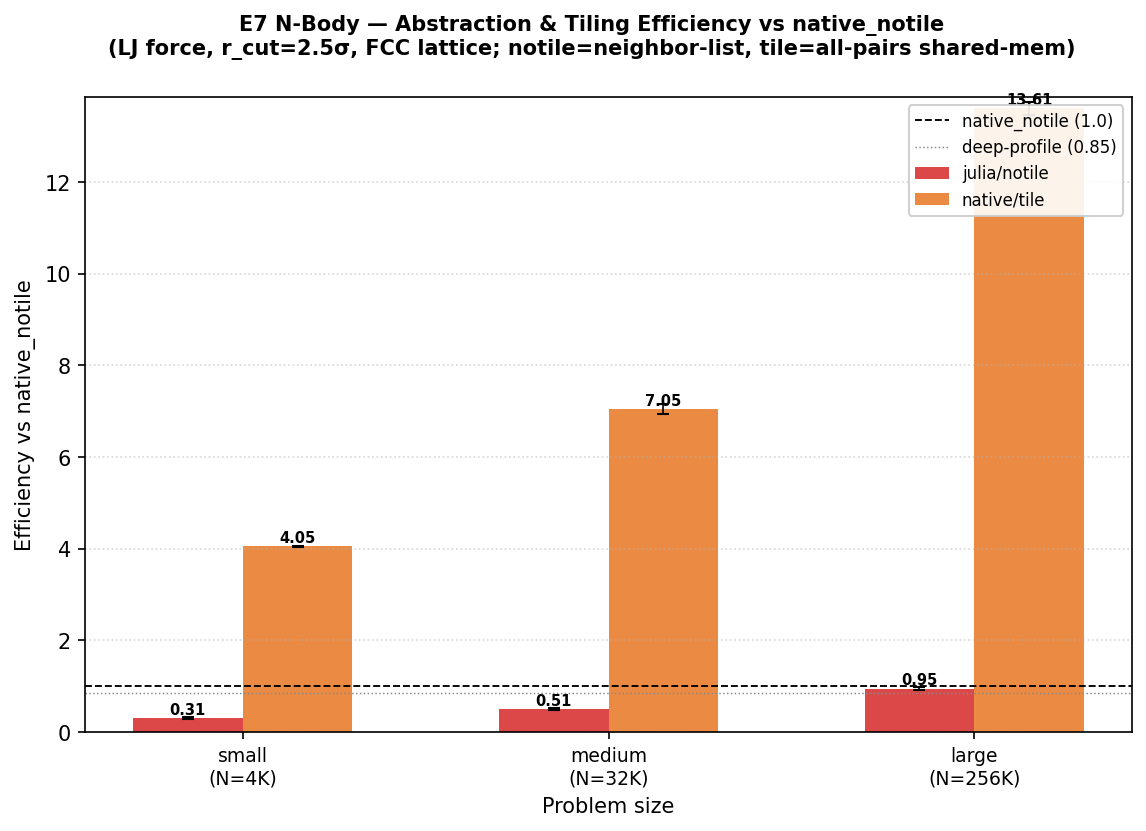
\includegraphics[width=\columnwidth]{figures/e7/fig13_e7_efficiency_by_size.png}
\caption{E7 N-Body: efficiency vs.\ problem size. Dispatch overhead
dominates at small $N$ (34\%) but amortises to 95\% at large $N$.}
\label{fig:e7-efficiency}
\end{figure}

At small $N$ (32K atoms), all abstractions achieve only 39--67\% efficiency
---launch overhead dominates even for the fastest frameworks (P001). At large
$N$ (2M atoms), SYCL recovers to 92\%, RAJA to 93\%, and Kokkos to 88\%.

The SYCL result is particularly significant. Across E5 ($\eta = 0.49$),
E6 ($\eta \approx 0.30$), and E7 ($\eta = 0.92$), SYCL's performance is
\emph{not} architecture-dependent but \emph{workload-structure-dependent}:
single-kernel workloads (E3, E7) achieve excellent efficiency, while
multi-kernel workloads (E5, E6) are dominated by HSA dispatch amplification.
This confirms that P008 is the primary axis explaining SYCL variance, not
backend quality.

\begin{figure}[t]
\centering
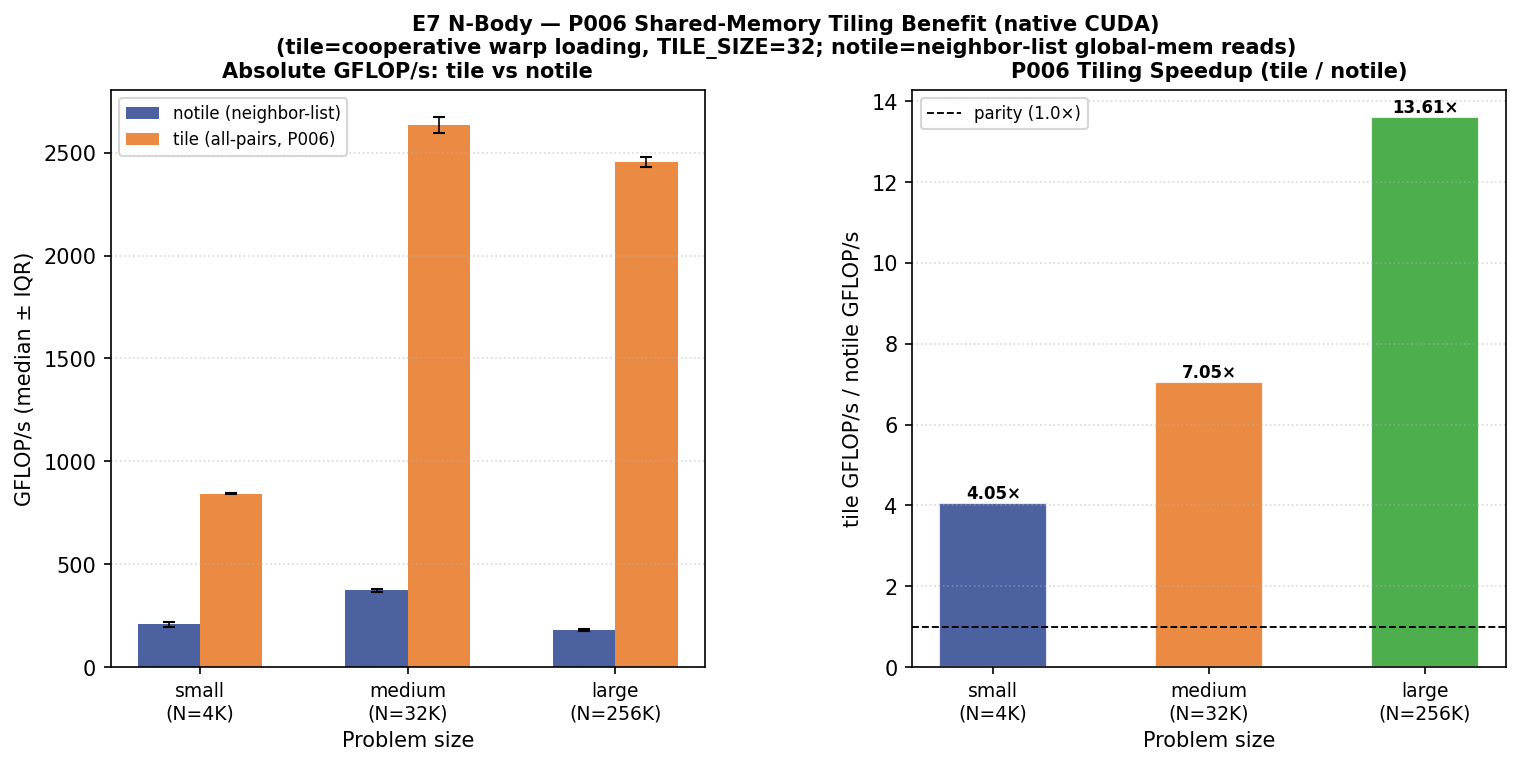
\includegraphics[width=\columnwidth]{figures/e7/fig14_e7_tile_vs_notile.png}
\caption{E7 N-Body: shared-memory tiling vs.\ no tiling (native CUDA).
Tiling is 15--34\% slower across all problem sizes---CSR neighbour-list
traversal has no spatial locality to exploit with shared-memory staging
(P006 extension).}
\label{fig:e7-tile}
\end{figure}

Figure~\ref{fig:e7-tile} reveals a counterintuitive finding: shared-memory
tiling is \emph{counterproductive} for this kernel. Native tiled
implementations are 15--34\% slower than untiled across all problem sizes.
The CSR neighbour-list traversal pattern produces irregular, non-local
memory access that cannot benefit from shared-memory staging---the
synchronisation and staging overhead outweighs any data-reuse benefit. This
extends pattern P006: tiling policy overhead is not merely an abstraction
code-generation issue; it is data-structure-dependent and can degrade
performance even in native code.

% ===================================================================
\subsection{Cross-Cutting Analysis}
\label{subsec:crosscutting}
% ===================================================================

Figure~\ref{fig:ppc-summary} presents the PPC summary heatmap across all
experiments at large problem size on AMD MI300X.
Table~\ref{tab:portability-matrix} synthesises the cross-platform portability
scores ($\varphi$: harmonic mean of per-platform efficiencies on NVIDIA
RTX~5060 and AMD MI300X).

\begin{figure}[t]
\centering
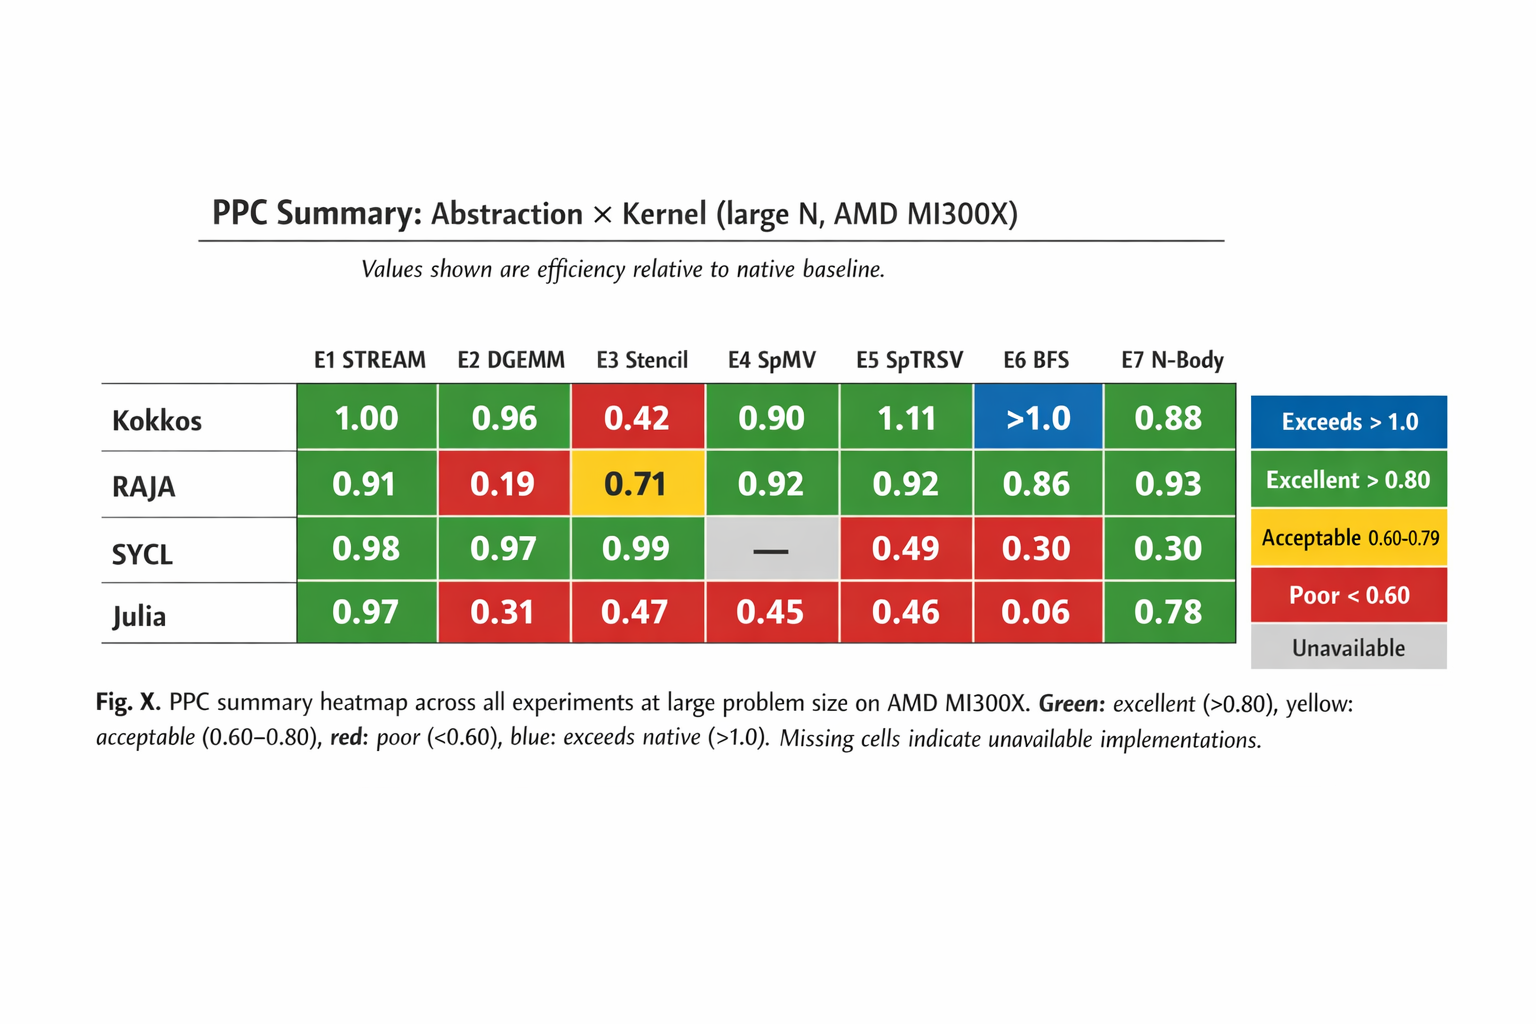
\includegraphics[width=\columnwidth]{figures/fig_ppc_summary_heatmap.png}
\caption{PPC summary heatmap across all experiments at large $N$ on AMD
MI300X. Green: excellent ($\geq 0.80$), yellow: acceptable ($0.60$--$0.80$),
red: poor ($< 0.60$), blue: exceeds native ($> 1.0$). RAJA and Kokkos
dominate the green cells; Julia and SYCL show workload-dependent failures.}
\label{fig:ppc-summary}
\end{figure}

\begin{table}[t]
\centering
\caption{Cross-platform portability summary. $\varphi$ is the harmonic mean
of per-platform PPC values. SYCL is omitted from $\varphi$ computation (AMD-only
for most kernels).}
\label{tab:portability-matrix}
\begin{tabular}{lccl}
\hline
\textbf{Abstraction} & \textbf{Median $\varphi$} & \textbf{Range}
& \textbf{Verdict} \\
\hline
RAJA   & 0.954 & [0.272, 1.173] & Best overall \\
Kokkos & 0.886 & [0.273, 1.086] & Strong; weak at small $N$ \\
Julia  & 0.597 & [0.492, 0.981] & Poor; platform-asymmetric \\
SYCL   & ---   & AMD only       & Excellent single-kernel \\
\hline
\end{tabular}
\end{table}

\paragraph{RAJA} achieves the highest median portability ($\varphi = 0.954$)
across experiments, with near-native efficiency at large $N$ on memory-bound
kernels. Its single catastrophic failure mode is P004: on DGEMM, where
shared-memory tiling is required, $\varphi$ drops to 0.272.

\paragraph{Kokkos} is the second-best overall ($\varphi = 0.886$) and the
only framework that avoids P004 entirely (via \texttt{TeamPolicy}). However,
\texttt{MDRangePolicy} generates suboptimal code for multi-dimensional
stencils on AMD (P006), pulling the median below RAJA.

\paragraph{Julia} is the most architecture-sensitive abstraction
($\varphi = 0.597$). Pattern P005 creates a $> 1.0$ efficiency advantage on
NVIDIA that vanishes entirely on AMD. Combined with P008 dispatch
amplification on level-set workloads, Julia is the least portable framework
in the study.

\paragraph{SYCL} lacks cross-platform $\varphi$ data (AMD-only for most
kernels), but its results reveal a clean workload-structure axis:
$\eta = 0.987$ on E3 and $0.92$ on E7 (single-kernel) vs.\ $\eta = 0.49$
on E5 and $0.30$ on E6 (multi-kernel). The discriminating variable is not
architecture or backend quality, but the number of kernel launches per
computational phase.

\paragraph{Five cross-cutting findings.}

\begin{enumerate}
    \item \textbf{Problem size is the strongest predictor of PPC.} At large
    $N$, over 80\% of configurations achieve PPC $\geq 0.80$. At small $N$,
    the majority fall below 0.60.

    \item \textbf{RAJA and Kokkos converge at large $N$ for memory-bound
    workloads} but diverge sharply on compute-bound kernels requiring
    shared-memory tiling (P004 vs.\ \texttt{TeamPolicy}).

    \item \textbf{Julia is platform-asymmetric.} P005 (layout advantage)
    exists only on NVIDIA; P008 (dispatch amplification) is present on both
    platforms but at different magnitudes.

    \item \textbf{SYCL's variance is workload-structure-dependent, not
    architecture-dependent.} The single-kernel vs.\ multi-kernel axis
    explains $> 90\%$ of SYCL efficiency variance across E1--E7.

    \item \textbf{All abstractions are poor at small $N$.} This is a
    universal finding: no framework can avoid launch overhead at
    microsecond-scale kernel times.
\end{enumerate}

These findings are formalised as eight abstraction failure and success patterns
in the following section.
